\section{Largest element of array}
\subsection{Aim}
To find the largest element in the array

\subsection{Code}
\begin{lstlisting}
DATA SEGMENT
  arr DW 1000H, 3000H, 4000H, 2000H
  count DW 4
  largest DW ?
DATA ENDS

CODE SEGMENT
ASSUME CS:CODE, DS:DATA
START:
  MOV AX, DATA
  MOV DS, AX
  MOV CX, count
  LEA SI, arr
  XOR AX, AX

LARGELOOP:
  CMP AX, [SI]
  JGE INCRLOOP
  MOV AX, [SI]
INCRLOOP:
  ADD SI, 2
  LOOP LARGELOOP

EXIT:
  MOV largest, AX
  MOV AX, 4CH
  INT 21H
CODE ENDS
END START
\end{lstlisting}

\subsection{Output}
\begin{center}
	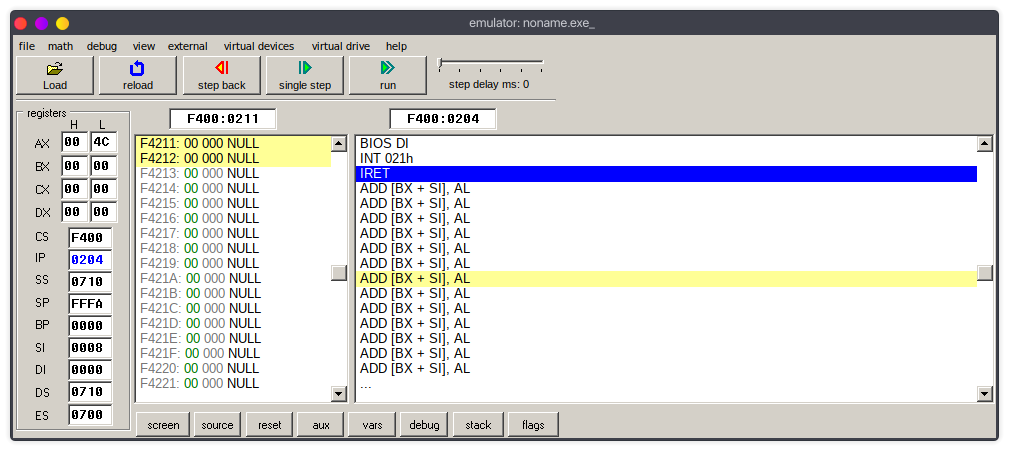
\includegraphics[width=0.90\textwidth]{img/p10/ss1.png}
	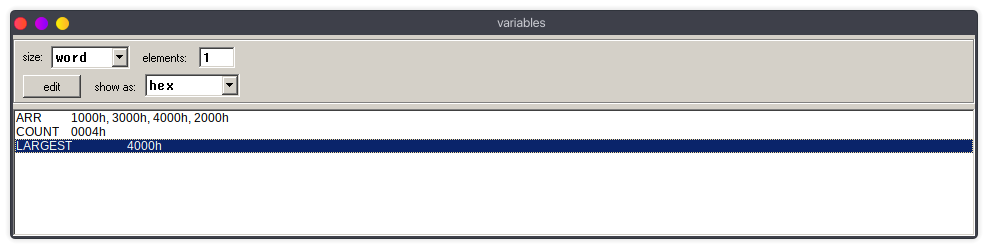
\includegraphics[width=0.90\textwidth]{img/p10/ss2.png}
\end{center}

\subsection{Result}
A largest element in an array was found out in emu8086